\documentclass[a4paper,10pt,twocolumn]{article}

\usepackage{inputenc}
\usepackage{float}
\usepackage{fontenc}
\usepackage{textcomp}
\usepackage{amsmath, amssymb}
\usepackage{graphicx}
\usepackage[width = 18cm,height = 22cm,columnsep = 1cm,margin = 2cm]{geometry}
\usepackage[backend=biber,style=authoryear]{biblatex}
\usepackage{aas_macros}
\usepackage{hyperref}
\hypersetup{
	colorlinks=true,
	linkcolor=blue,
	citecolor=blue,
	urlcolor=cyan,
	pdftitle={Sloan Digital Sky Survey Software Development: Week 9 Progress Report},
	pdfpagemode=FullScreen,
}

\bibliography{/home/riley/rproj/reports/w9/bibliography.bib}
\graphicspath{{/home/riley/rproj/reports/w9/images/}}

\title{Sloan Digital Sky Survey Software Development}
\author{Riley Thai, Andy Casey (Supervisor)}
\setcounter{secnumdepth}{4}
\makeatletter
\renewcommand\paragraph{\@startsection{paragraph}{4}{\z@}%
	% display heading, like subsubsection
	{-3.25ex\@plus -1ex \@minus -.2ex}%
	{1.5ex \@plus .2ex}%
	{\normalfont\normalsize\bfseries}}
\setcounter{secnumdepth}{4}
\makeatother

\newcommand{\solara}{\texttt{solara}}
\newcommand{\vaex}{\texttt{vaex}}
\newcommand{\specutils}{\texttt{specutils}}
\newcommand{\jdaviz}{\texttt{jdaviz}}
\newcommand{\visboard}{\emph{Visboard}}

\begin{document}
\twocolumn[
	\begin{@twocolumnfalse}
		\maketitle
		\begin{abstract}
			We developed a new, multi-dimensional parameter explorer web application, named the \emph{Visboard} for online data exploration of the upcoming largest Data Release of the Sloan Digital Sky Survey (SDSS). We also developed default loaders for \specutils\, allowing for new datatypes in the fifth-generation SDSS data releases to be loaded directly as Python objects for manipulation with other libraries, such as \jdaviz. In this report, we showcase the key features of these software application, the design decisions made, and discuss the future plans for the development of the \emph{Visboard}.
		\end{abstract}
		% add spaces as necessary
		$\,$
		%$\,$
	\end{@twocolumnfalse}]

\section{Introduction}
Astronomers run observation programs called ``surveys" to determine the properties of a large number of objects, from the stellar parameters and abundances of stars, to the accretion rate of black holes. By providing large catalogs of objects, astronomers and astrophysicists alike can explore these datasets to test their hypotheses, validate the results of others, and develop our understanding of the universe at large.

The Sloan Digital Sky Survey (SDSS) is one of the largest, longest running, and most used astronomical surveys. Started in 1998 \parencite{dr18}, the SDSS provides all-sky, multi-epoch spectroscopy using telescopes in both hemispheres, providing data used to probe the emergence of chemical elements, reveal the inner mechanisms of stars, and investigate the origin of planets. The latest generation of the survey, SDSS-V, aims to conduct the first homogeneous survey using an optical, ultra-wide integral-field spectroscopic map of the interstellar gas, pioneering spectroscopic monitoring and revealing changes on both short and vast timescales \parencite{SDSS2017}. SDSS data over all survey phases has been cited more than 650,000 over 111,000 refereed papers \parencite{dr18}.

The fifth generation of the survey, SDSS-V,  The latest generation of the survey, SDSS-V, aims to conduct the first homogeneous survey using an optical and infrared (IR), ultra-wide integral-field spectroscopic map of the interstellar gas, pioneering spectroscopic monitoring and revealing changes on both short and vast timescales \parencite{SDSS2017}. The survey's key scientific goals are bundled into three different programs.

\begin{figure}[htpb]
	\centering
	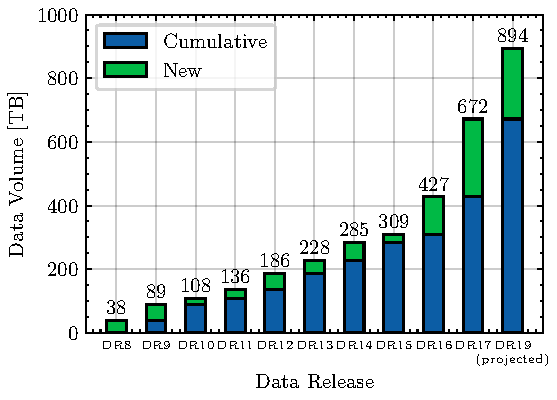
\includegraphics[width=1.0\columnwidth]{datavolhist}
	\caption{A histogram of the cumulative data volume of each Data Release of the SDSS since Data Release 8 (DR8). The next Data Release, DR19, is projected to have 1.3x the amount of data in Data Release 17, with the cumulative data volume totalling to possibly over 900 terabytes.}
	\label{fig:datavols}
\end{figure}
The Milky Way Mapper (MWM) will employ both optical and near-IR spectroscopy across over 5 million stellar objects, providing a dense, contiguous map of the sky with a high-dimensional parameter space, including stellar mass, age, chemical composition, rotation, and internal structure. The MWM aims to recreate the deep history of the Milky Way Galaxy through quantitive tests of physics-based galactic formation models against its large, high-dimensional catalog \parencite{SDSS2017}.

The Black Hole Mapper (BHM) studies quasars and their supermassive black holes (SMBHs) at the center of galaxies to trace the evolution of BHs across cosmic timescales \parencite{SDSS2017}. Through optical spectroscopy, the BHM will provide mass measures and multi-wavelength spectral energy distributions for a large sample of over 300,000 quasars, developing insight into the co-evolution of SMBHs with their host galaxies.

\begin{figure*}[t]
	\centering
	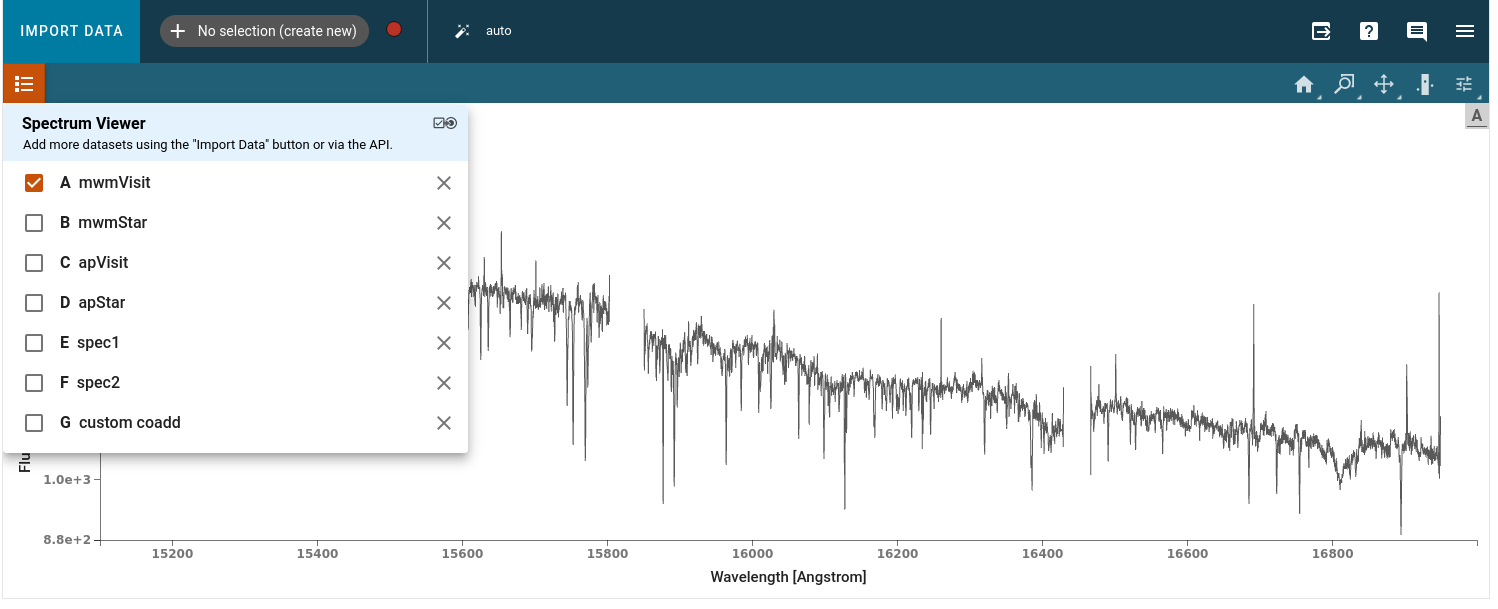
\includegraphics[width=0.9\textwidth]{jdaviz}
	\caption{Spectrum data from a BOSS spectrograph, as shown within \jdaviz\, SpectrumViewer. Note that other spectra are also loaded, and can be toggled by the checkbox.}
	\label{fig:jdaviz}
\end{figure*}

The Local Volume Mapper (LVM) aims to study the self-regulating processes of galactic formation by creating global interstellar medium (ISM) maps of Local Group galaxies and nebulae through high-resolution telescopes and spectrographs \parencite{SDSS2017}. The LVM will return data aimed at researching star formation and the physics of the ISM through revealing individual star formation knots and the shock networks of filamentary structures across local nebulae and galaxies.

With the large number of new scientific goals, the total data volume of the survey has increased dramatically, as shown in Figure \ref{fig:datavols}. The SDSS has previously offered a simple web application for end users to access, explore, and investigate spectra and data catalogs. However, since the fifth generation of the survey is offering a massive, high-dimensional catalog of several different types of galactic objects, there is a need for a new tool which provides powerful exploration and visualization of large and vast datasets without a user needing to download the extremely large dataset locally.

In this report, we detail the development work undertaken and software features of a multi-dimensional, out-of-core parameter explorer for SDSS data, alongside the implementation of automatic loaders for SDSS datatypes within the Python library \specutils. In Section \ref{sec:specutils}, we describe the features implemented into \specutils\, and the utility they provide. In Section \ref{sec:visboard}, we showcase and outline the Parameter Explorer and its features, describing the design decisions and the key software functionality. Finally, we outline our future plans in Section \ref{sec:future}, and write our conclusions in Section \ref{sec:conclusion}.


\section{\texttt{specutils} Default Loaders}
\label{sec:specutils}
The Python library \specutils\, is package which provides a Python object representation of spectra and basic operation tools \parencite{specutils}. The package is part of the Astropy project, which aims to provide a centralized and widely applicable set of tools for handling astronomical data \parencite{astropyarticle}. Of note is its integration with spectrum viewers and analysis tools, such as the \jdaviz\, package, which provides data viewers and analysis plugins for interactive applications \parencite{jdavizarticle}.

Of use to the SDSS collaboration and the wider public would be the feature to automatically load the new and updated SDSS datatypes with \specutils\, spectrum representations, namely the \texttt{Spectrum1D}\, and \texttt{SpectrumList}\, objects.

As such, the software I developed provides default I/O reading functions for both the new and updated datatypes within the SDSS-V dataset. There were changes to the location of wavelength and spectral flux properties within the \texttt{apStar}, \texttt{apVisit}, and SDSS \texttt{spec}\, datatypes. It can handle loading spectra files both locally and via a direct web link directly as \texttt{Spectrum1D}\, or \texttt{SpectrumList}\, objects.

The handlers are built-in as the sub-method to each \texttt{Spectrum} class, by specifying a filepath, a user can also choose to read a single or all spectrum from a given SDSS data file.

Most importantly, other libraries which use the \texttt{Spectrum} objects to load the new SDSS-V datatypes, such as the \jdaviz\, spectrum viewer, can now read SDSS-V datatypes. Several loaded spectrum objects from SDSS-V spectra are shown in Figure \ref{fig:jdaviz}.


The pull request to merge this functionality into the \specutils\, package is currently under review, and can be viewed \href{https://github.com/astropy/specutils/pull/1107}{here} for further reading.

\section{Parameter Explorer}
\label{sec:visboard}
\begin{figure*}[t]
	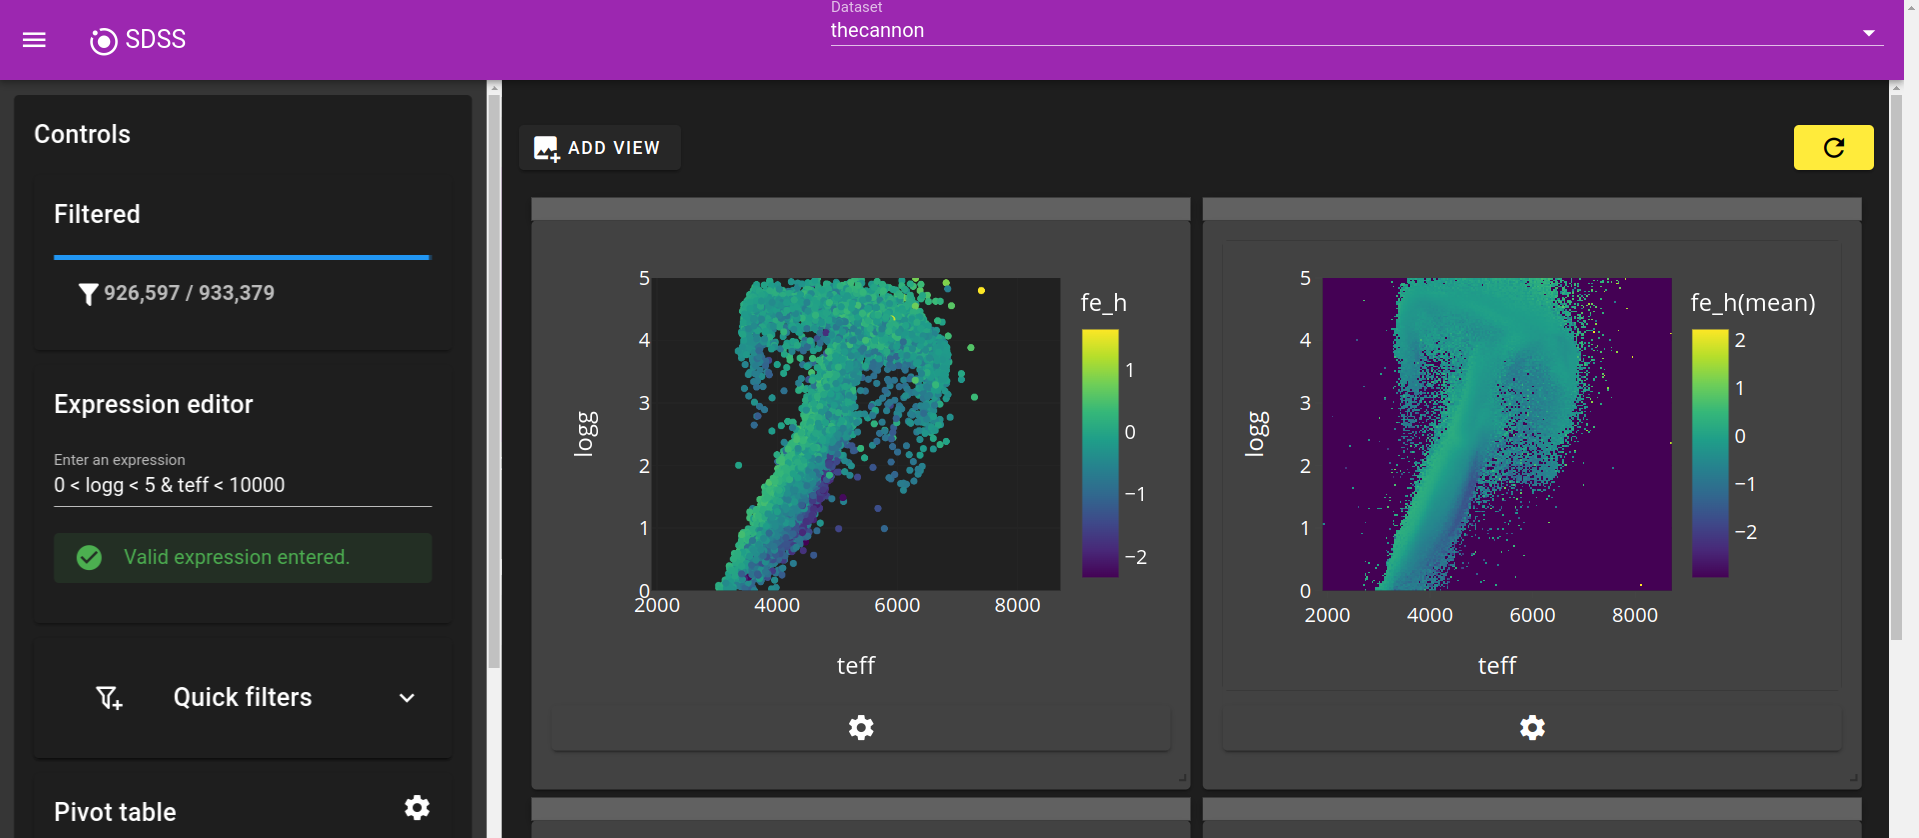
\includegraphics[width=1.0\textwidth]{wholeapp}
	\caption{A full screenshot of the application. Top: the Application bar, where the loaded dataset can be changed, currently viewing data from \emph{The Cannon} \parencite{thecannon}. Left: the sidebar, containing filter controls, such as the expression editor. An expression to filter out values is currently applied. Right: the sticky note layout, showing the scatter and aggregation views, plotting $T_{\mathrm{eff}}$ and $\log g$.}
	\label{fig:wholeapp}
\end{figure*}
The fifth generation of the SDSS now provides complete stellar labels across multiple different pipelines via the Astra framework. The Parameter Explorer, or the \visboard, is a in-development data webapp which will be hosted on SDSS servers and provide both public and proprietary SDSS data to its users for multi-dimensional data exploration.

The VisBoard provides data exploration across a variety of viewing forms through an intuitive user experience. Much like a board of sticky notes, views can be added, removed, and resized at will by the user, whilst applying global filters across the selected dataset. Views themselves are dynamic, rerendering to filter out unnecessary points and saving zoom and pan information for a smoother UX. Users can choose between different SDSS datasets, and

In Section \ref{sec:tech}, we discuss the software choices for the library and outline our reasoning. Throughout Section \ref{sec:features}, we discuss the key features of the application. In Section \ref{sec:sticky}, we discuss the application's sticky note layout, the plotting views, such as the aggregated (\ref{sec:aggregated}) and skyplot plots (\ref{sec:skyplot}), and the dynamic rerendering across these views in Section \ref{sec:rerender}. In Section \ref{sec:filter}, we discuss the application's cross-filtering functionality across all views and the user-facing dataset filtering, called Expressions. In Section \ref{sec:datasets}, we describe how the software supports multiple datasets and discuss future implementations of this functionality.

\subsection{Technology}
\label{sec:tech}
The \visboard\, utilizes various Python packages, as Python has become the premier language for astronomical analysis and data science. Three packages were core to the application's functionality.

\begin{enumerate}
	\item \solara\, -- a Python, React-like web application framework.
	\item \vaex\, -- a data science focused package for handling very large datasets out-of-core \parencite{vaex}.
	\item \texttt{Plotly.py} -- a highly interactive graphing and plotting library \parencite{plotly}.
\end{enumerate}

The choice for using \solara\, was experimental, but necessary. Released in 2022, the \solara\, library builds on existing technology, such as Vuetify components and the \texttt{ipywidgets}\, system. Being written in Python, it allows for high speed development workflows through easier integration with data science packages already written in Python, such as \vaex.

\vaex\, specifically is the fundamental core of the application's backend data processing, as it provides extremely fast aggregated statistics and out-of-core data handling. \vaex\, was specifically developed to handle a new era of big data astronomy, such as Gaia and the upcoming LVM data \parencite{vaex}, and is capable of handling upto over 1 billion rows of data. Futhermore, the data is encoded as a parquet file, which allows for high-speed in-memory processing and data interchange via the Apache Arrow columnar data layout \parencite{parquet}.

Finally, \texttt{Plotly.py} was chosen as the visualization library due to its highly interactive components, which allow for distinct user hover information and interactive selections of the dataset.

The two other packages used were \texttt{numpy} \parencite{numpy} and \texttt{xarray} \parencite{xarray}, which provided several quantitative data calculation methods.

\begin{figure}[tp]
	\centering
	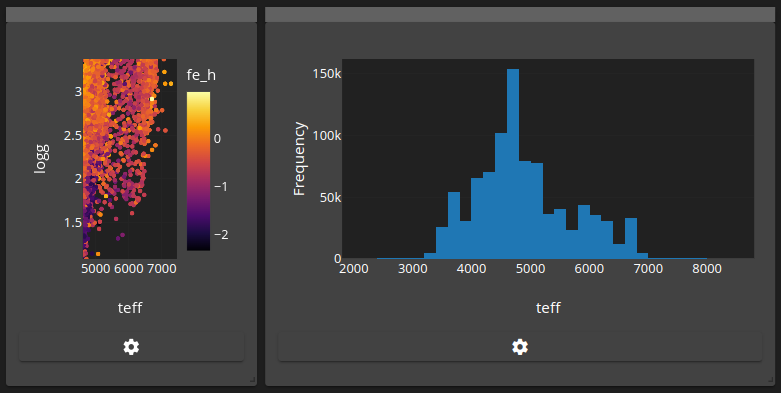
\includegraphics[width=1.0\columnwidth]{layout}
	\caption{A demonstration of the dynamic resizing and draggable view ``notes". The plot objects dynamically resize to fit their container, and can be rearranged and resized by the user with their mouse.}
	\label{fig:layout}
\end{figure}


\subsection{Application Features}
\label{sec:features}
\subsubsection{Layout and Views}
\label{sec:sticky}
The user can directly add and remove multiple plotting views of the same time within their display, which can resized with a small handle in the bottom right, and moved via the top grey toolbar, as shown in Figure \ref{fig:wholeapp}. Each plot also dynamically resizes to its containing ``note", which can be seen in Figure \ref{fig:layout}.

There are 5 different views with can be added to the layout -- histogram, scatter, aggregated, skyplot, and table views.

Within each view, a plot's individual properties can be changed, such as colorscale, the data to plot, and whether a given axis is flipped and/or logarithmic scale, as shown in Figure \ref{fig:skyplot}.

Each view has a selection option, which allows the user to select certain bins, points, or rows, which will then be cross filtered to other open views.

On the scatter plot views, a user can right click on any given star to directly download the spectrum of that object, or view the object's spectra via \texttt{jdaviz}. Currently, these lead to placeholders, but will eventually be replaced with browser links to the public SDSS data by the ID lookup.

\paragraph{Aggregated}
\label{sec:aggregated}
The aggregated view utilizes an image render based on Plotly's \texttt{imshow} to provide a high detail 3 dimensional view. By utilizing \vaex's aggregated statistics over n-dimensional grids, which allows for complex multi-dimensional plotting, the view bypasses the pitfalls of scatter plots, such as overplotting or underrepresentation through downsampling. This view is shown in Figure \ref{fig:2d}.

The view can show the mean, minimum, maximum, or mode of any cell on the grid, and the size of the grid can be adjusted.

\begin{figure}[tp]
	\centering
	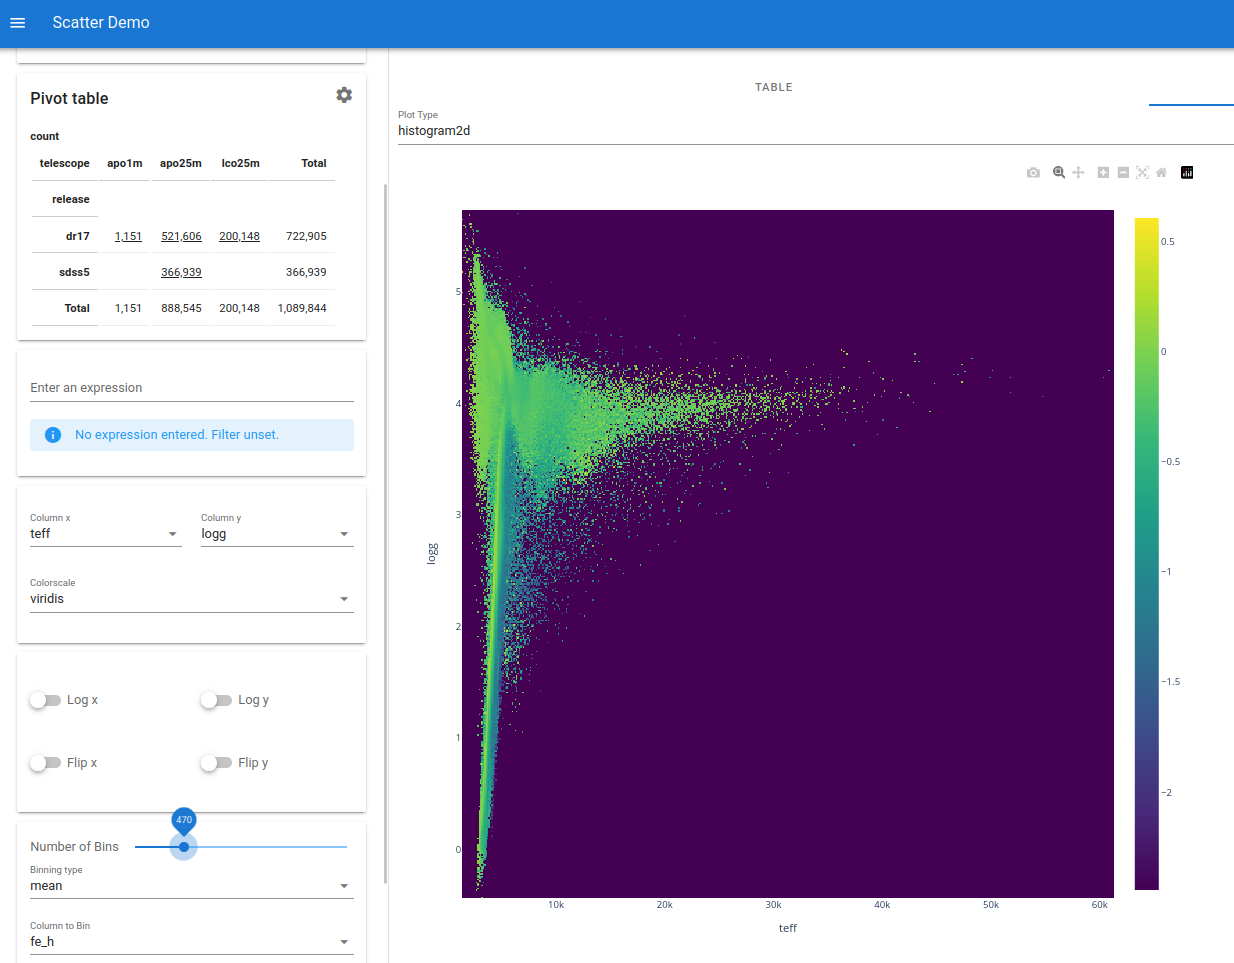
\includegraphics[width=\columnwidth]{2d}
	\caption{A display showing the aggregated view, plotting the ASPCAP catalog objects' effective temperature $T_{\mathrm{eff} }$ vs. surface gravity $\log g$, colored by the mean metallicity $\mathrm{[Fe / H]} $. The axes are inverted.}
	\label{fig:2d}
\end{figure}

\paragraph{Skyplot}
\label{sec:skyplot}
The skyplot is a scatter plot with a sky projection, herein referred to as a ``\emph{skyplot}". This view was heavily requested by astronomers after consultations and demonstrations. The user can switch between plotting right ascension vs. declination ($\mathrm{RA / DEC} $) or galactic longitude and latitude ($l / b $). Panning the view will accurately map the points according to the projection type, which can be set by the user. The settings menu and skyplot are shown in Figure \ref{fig:skyplot}


\paragraph{Dynamic rerendering and filtering}
\label{sec:rerender}
Another new feature is the adaptive rerendering of Plotly's \texttt{FigureWidget} objects, which consists of two parts:
\begin{enumerate}
	\item Rerendering the plot with the same zoom and pan settings after a parameter change.
	\item Filtering the dataset in the Scatter object views (\emph{skyplot} + \emph{scatter}) to the ranges of the zoomed plot in real time.
\end{enumerate}

In previous versions, the plot would forcibly reset after any parameter change, such as changing the colorscale or binning type, which led to a disorienting UX that required the user to continuously redo their zoom/pan actions after parameter changes. Now, the plot continuously saves the visible x/y ranges, and calls upon them when plotting, only resetting it if the x/y data or plotting scale changes.

The other consequence of saving the relayout information is that it allows for us to directly filter the dataset to only include data inside the visible range, which allows the user to see more points after performing zoom or pan operations, bypassing the overplotting limitations of Plotly's memory-heavy scatter points. This allows for us to have an effectively infinite zoom with complete hover information, allowing for precise dataset exploration across bot the scatter and skyplot views. This is similar in function to Holoview's \texttt{DataShader} \parencite{holoviews}, although we do not rasterize the data prior to plotting.

\subsubsection{Cross-filtering}
\label{sec:filter}
Within the application's sidebar on the left hand side (see Figure \ref{fig:wholeapp}), one can access dataset filtering controls, such as an Expression Editor, Quick Filters, and a Pivot Table.

The Expression Editor allows the user to leverage \vaex 's high-speed computations to filter the dataset. This can be combined with other filtering methods, the pivot table and/or selection, to directly select a complex subset of data. A truncated view containing the Expression Editor is shown in Figure \ref{fig:sidebar}.

\begin{figure}[tp]
	\centering
	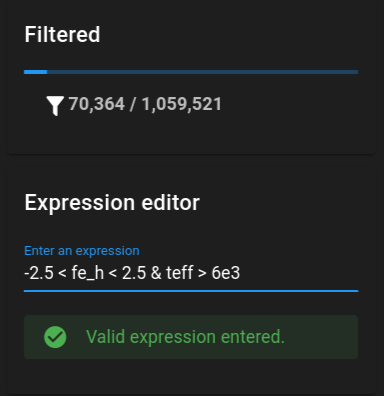
\includegraphics[width=\columnwidth]{sidebar}
	\caption{A truncated view of the sidebar of the explorer, with an Expression applied to the dataset. Top: The number of rows in the current filtered dataset. Bottom: The expression editor.}
	\label{fig:sidebar}
\end{figure}

The Quick Filter menu contains checkboxes to quickly apply common filters. This was a feature suggested by astronomers after demonstrations within SDSS telecons. Currently, it is implemented with the basic functionality to limit the dataset to high SNR subsets ($\mathrm{SNR} >50$), or only include non-flagged results. The functionality can be expanded in future to potentially hold user filters, or alternatively limit to different cartons.

The Pivot Table also allows a user to filter the dataset based on a specific result in a distinct UI, powered by \vaex's groupby objects. Users can click on a given set of the data to filter the dataset to that row, column, or cell of the pivot table. The user's subset of the chosen dataset can also be directly downloaded, based on their chosen filters. The pivot table is shown in Figure \ref{fig:pivottable}.

\begin{figure}[tp]
	\centering
	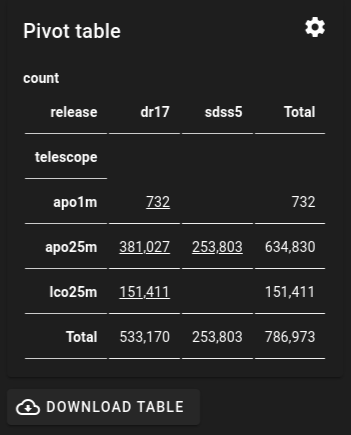
\includegraphics[width=\columnwidth]{pivottable}
	\caption{A view of the pivot table, showcasing release vertically, and telescope horizontally. Users can click on a given set of the data to filter the dataset down to that row, column, or cell of the pivot table. Further specifications can be added by the cog icon in the top right.}
	\label{fig:pivottable}
\end{figure}


\subsubsection{Multiple Datasets}
\label{sec:datasets}
Within the top left of the application, the user can now directly select the Astra pipeline from which to access data from (see top of Figure \ref{fig:wholeapp}).

Currently, this is implemented as a proof-of-concept feature, with the goal being to allow a user to select multiple pipeline datasets simultaneously, and apply unique filters and expressions directly between them or across all of them, and even their own given subsets.
The exact implementation of this feature and method depends on how data will be stored across different access methods, which is yet to be decided as it depends on the data volume organization and pipeline output frequency for the working dataset and the public Data Release.

As shown previously, the user's subset of the chosen dataset can also be directly downloaded, based on their chosen filters.
\begin{figure}[tp]
	\centering
	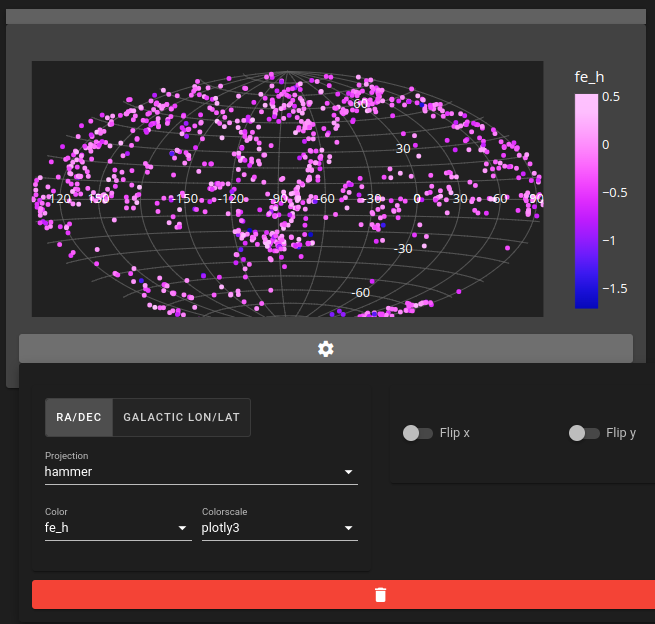
\includegraphics[width=1.0\columnwidth]{skyplot}
	\caption{Top: the \emph{skyplot} view, showing right ascension (RA) against declination (DEC), and colored by metallicity $\mathrm{[Fe / H]}$ across a Hammer projection. Bottom: the settings menu of the skyplot view, where the coordinates, projection type, color values, colorscale, and axes flips can be changed by the user.}
	\label{fig:skyplot}
\end{figure}

\section{Future Plans}
\label{sec:future}
While the majority of core development features are completed, there is still work required to expand its functionality, polish the application, and improve its performance.

Since the user experience is of vital importance, we seek to present this application to the collaboration several more times before the launch of Data Release 19 in late 2024 for feedback. Their input is vital for understanding the scientific workflow and the necessary tools and integrations. Currently, suggested ideas have included the multiple dataset functionality, saving and loading different filters, quick carton-based filtering, and accessibility improvements, such as font sizes and colorblind-accessible colorscale palettes.

To allow for users to understand the application thoroughly, we plan to develop a deployable container on an SDSS server, so users can use the application in their own time for their own science or testing. The Data Visualization group within the SDSS Collaboration will soon be granted access to a virtual machine (VM) for testing and developing applications. Members of the collaboration are interested in providing feedback and testing the application, and have suggested using \texttt{Singularity} \parencite{singularity} as the portable app-container for the development workflow.

Some other key features we are looking to implement are the loading of several datasets simultaneously from different pipelines, such as loading an ASPCAP and ApogeeNET dataset simultaneously, which will help with pipeline performance assessment. We also plan to expand upon \texttt{vaex}'s features to provide lazy, out-of-memory computations, such as virtual columns based on user calculations.

The performance of the application has decreased since earlier versions. This is due to the number of components, callbacks, and hooks increasing dramatically without proper state co-location and memoization, which can prevent unnecessary rerenders. The codebase must be revised to ensure that the application doesn't perform these rerenders and other variable checks, especially with regards to the plotting code.

There are also still numerous bugs, which will be resolved in course through the continued development of the application.

\section{Conclusion}
\label{sec:conclusion}
\textbf{No idea what to do here -- does this style of report even need one?}

\section*{Special Thanks}
I thank Andy Casey, my supervisor, for his assistance with this project. Specifically, I thank him for permitting me to work fully remotely with minimal overhead supervision.

I would like to thank Brian Cherinka and Joel Brownstein of the SDSS Collaboration/University of Baltimore for providing me with this opportunity to work on this project.

I also extend my thanks to the Data Visualization Group and Astra Group of the working SDSS Collaboration, for their feedback and support through the development of this application.
\printbibliography

\end{document}


